\documentclass[a4paper,11pt,fleqn,twoside,notitlepage]{report}
\usepackage[]{graphicx}\usepackage[]{color}
%% maxwidth is the original width if it is less than linewidth
%% otherwise use linewidth (to make sure the graphics do not exceed the margin)
\makeatletter
\def\maxwidth{ %
  \ifdim\Gin@nat@width>\linewidth
    \linewidth
  \else
    \Gin@nat@width
  \fi
}
\makeatother

\definecolor{fgcolor}{rgb}{0.345, 0.345, 0.345}
\newcommand{\hlnum}[1]{\textcolor[rgb]{0.686,0.059,0.569}{#1}}%
\newcommand{\hlstr}[1]{\textcolor[rgb]{0.192,0.494,0.8}{#1}}%
\newcommand{\hlcom}[1]{\textcolor[rgb]{0.678,0.584,0.686}{\textit{#1}}}%
\newcommand{\hlopt}[1]{\textcolor[rgb]{0,0,0}{#1}}%
\newcommand{\hlstd}[1]{\textcolor[rgb]{0.345,0.345,0.345}{#1}}%
\newcommand{\hlkwa}[1]{\textcolor[rgb]{0.161,0.373,0.58}{\textbf{#1}}}%
\newcommand{\hlkwb}[1]{\textcolor[rgb]{0.69,0.353,0.396}{#1}}%
\newcommand{\hlkwc}[1]{\textcolor[rgb]{0.333,0.667,0.333}{#1}}%
\newcommand{\hlkwd}[1]{\textcolor[rgb]{0.737,0.353,0.396}{\textbf{#1}}}%

\usepackage{framed}
\makeatletter
\newenvironment{kframe}{%
 \def\at@end@of@kframe{}%
 \ifinner\ifhmode%
  \def\at@end@of@kframe{\end{minipage}}%
  \begin{minipage}{\columnwidth}%
 \fi\fi%
 \def\FrameCommand##1{\hskip\@totalleftmargin \hskip-\fboxsep
 \colorbox{shadecolor}{##1}\hskip-\fboxsep
     % There is no \\@totalrightmargin, so:
     \hskip-\linewidth \hskip-\@totalleftmargin \hskip\columnwidth}%
 \MakeFramed {\advance\hsize-\width
   \@totalleftmargin\z@ \linewidth\hsize
   \@setminipage}}%
 {\par\unskip\endMakeFramed%
 \at@end@of@kframe}
\makeatother

\definecolor{shadecolor}{rgb}{.97, .97, .97}
\definecolor{messagecolor}{rgb}{0, 0, 0}
\definecolor{warningcolor}{rgb}{1, 0, 1}
\definecolor{errorcolor}{rgb}{1, 0, 0}
\newenvironment{knitrout}{}{} % an empty environment to be redefined in TeX

\usepackage{alltt}
\newcommand{\SweaveOpts}[1]{}  % do not interfere with LaTeX
\newcommand{\SweaveInput}[1]{} % because they are not real TeX commands
\newcommand{\Sexpr}[1]{}       % will only be parsed by R


\setcounter{tocdepth}{3}
\setcounter{secnumdepth}{3}

\usepackage[utf8]{inputenc}
\usepackage[margin=2.5cm]{geometry}
\usepackage{graphicx}
\usepackage[T1]{fontenc}
\usepackage{enumitem}
\usepackage[section]{placeins}
\usepackage{csquotes}
\usepackage[english]{babel}
\usepackage{float}
\usepackage{caption}
\usepackage{makecell}
\usepackage{hyperref}
\usepackage{bm}
\usepackage{newfloat}
\usepackage[linesnumbered,lined,boxed,commentsnumbered]{algorithm2e}
\usepackage{booktabs}
\usepackage{colortbl}
\usepackage{tikz}

\usepackage{amssymb,amsmath,amsthm,amsfonts}
\newtheorem{theorem}{Theorem}

\usepackage{fancyhdr}
\setlength{\headheight}{15pt}

\pagestyle{fancy}
\renewcommand{\chaptermark}[1]{ \markboth{#1}{} }
\renewcommand{\sectionmark}[1]{ \markright{#1}{} }

\fancyhf{}
\fancyfoot[CE,CO]{\thepage}
\fancyhead[LE]{\textit{ \nouppercase{\leftmark}} }
\fancyhead[LO]{\textit{ \nouppercase{\rightmark}} }
%\fancyhead[RE,RO]{Erik Thors\'{e}n, \href{mailto:Ethorsn@gmail.com}{Ethorsn@gmail.com} }
\fancypagestyle{plain}{ %
\fancyhf{} % remove everything
  \renewcommand{\headrulewidth}{0pt} % remove lines as well
  \renewcommand{\footrulewidth}{0pt}
}

\usepackage[citestyle=authoryear,bibstyle=authoryear,natbib=true,backend=bibtex,hyperref=true,maxnames=2]{biblatex}

\bibliography{REFERENCES.bib}

\title{Statistical process control in next-generation sequencing quality control data}
\author{Erik Thors\'{e}n \thanks{Postal adress: Mathematical Statistics, Stockholm University, SE-106 91, Sweden. E-mail: Ethorsn@gmail.com. Supervisors: Taras Bodnar and Johan Dahlberg}}
\date{\today}

\raggedbottom


\begin{document}

\begin{knitrout}
\definecolor{shadecolor}{rgb}{0.969, 0.969, 0.969}\color{fgcolor}\begin{kframe}
\begin{alltt}
\hlcom{#Libraries}
\hlkwd{library}\hlstd{(Rcpp)}
\hlkwd{library}\hlstd{(RcppArmadillo)}
\hlkwd{library}\hlstd{(ggplot2)}
\hlkwd{library}\hlstd{(reshape2)}
\hlkwd{library}\hlstd{(GGally)}
\hlkwd{library}\hlstd{(lubridate)}
\hlkwd{library}\hlstd{(tidyr)}
\hlkwd{library}\hlstd{(dplyr)}
\end{alltt}


{\ttfamily\noindent\itshape\color{messagecolor}{\#\# \\\#\# Attaching package: 'dplyr'}}

{\ttfamily\noindent\itshape\color{messagecolor}{\#\# The following objects are masked from 'package:lubridate':\\\#\# \\\#\#\ \ \ \  intersect, setdiff, union}}

{\ttfamily\noindent\itshape\color{messagecolor}{\#\# The following object is masked from 'package:GGally':\\\#\# \\\#\#\ \ \ \  nasa}}

{\ttfamily\noindent\itshape\color{messagecolor}{\#\# The following objects are masked from 'package:stats':\\\#\# \\\#\#\ \ \ \  filter, lag}}

{\ttfamily\noindent\itshape\color{messagecolor}{\#\# The following objects are masked from 'package:base':\\\#\# \\\#\#\ \ \ \  intersect, setdiff, setequal, union}}\begin{alltt}
\hlkwd{library}\hlstd{(portes)}
\end{alltt}


{\ttfamily\noindent\itshape\color{messagecolor}{\#\# Loading required package: parallel}}\begin{alltt}
\hlkwd{library}\hlstd{(car)}
\hlkwd{library}\hlstd{(gridExtra)}
\hlkwd{library}\hlstd{(grid)}
\hlkwd{library}\hlstd{(ggExtra)}
\hlkwd{library}\hlstd{(parallel)}
\hlkwd{library}\hlstd{(xtable)}
\hlcom{# Load all data that is necessary}
\hlkwd{load}\hlstd{(}\hlstr{"../Data/meanH.Rdata"}\hlstd{)}
\hlkwd{load}\hlstd{(}\hlstr{"../Data/WishartH.Rdata"}\hlstd{)}
\hlkwd{load}\hlstd{(}\hlstr{"../Data/ICdata.Rdata"}\hlstd{)}
\hlkwd{load}\hlstd{(}\hlstr{"../Data/LambdaAndXtable.Rdata"}\hlstd{)}
\hlcom{# IC parameters}
\hlstd{K} \hlkwb{<-} \hlnum{100}
\hlstd{OrgOrder} \hlkwb{<-} \hlkwd{colnames}\hlstd{(TransformedData)}
\hlcom{# divide by a constant!}
\hlstd{TransformedData[,}\hlnum{1}\hlopt{:}\hlkwd{ncol}\hlstd{(TransformedData)} \hlopt \hlkwd{grep}\hlstd{(}\hlstr{"mean"}\hlstd{,OrgOrder)]} \hlkwb{<-} \hlstd{TransformedData[,}\hlnum{1}\hlopt{:}\hlkwd{ncol}\hlstd{(TransformedData)} \hlopt \hlkwd{grep}\hlstd{(}\hlstr{"mean"}\hlstd{,OrgOrder)]}\hlopt{/}\hlstd{K}

\hlstd{M} \hlkwb{<-} \hlkwd{nrow}\hlstd{(TransformedData)}

\hlstd{mu0} \hlkwb{<-} \hlkwd{colMeans}\hlstd{(TransformedData)}
\hlstd{Sigma0} \hlkwb{<-} \hlkwd{var}\hlstd{(TransformedData)}\hlopt{*}\hlstd{(M}\hlopt{-}\hlnum{1}\hlstd{)}\hlopt{/}\hlstd{M}

\hlcom{# R functions and scripts.}
\hlkwd{load}\hlstd{(}\hlstr{"../Data/MySQL_data.Rdata"}\hlstd{)}
\hlstd{All.df.reduced} \hlkwb{<-} \hlkwd{filter}\hlstd{(All.df.reduced,}\hlkwd{year}\hlstd{(Date)}\hlopt{>}\hlnum{2012}\hlstd{)}
\hlkwd{source}\hlstd{(}\hlstr{"../FunctionsAndRcpp/BotlvlSeriesExtraction.R"}\hlstd{)}
\hlcom{# C++ Functions}
\hlkwd{sourceCpp}\hlstd{(}\hlstr{"../FunctionsAndRcpp/RcppCPDestimation.cpp"}\hlstd{,}\hlkwc{showOutput}\hlstd{=}\hlnum{FALSE}\hlstd{,} \hlkwc{verbose} \hlstd{=} \hlnum{FALSE}\hlstd{)}
\hlkwd{sourceCpp}\hlstd{(}\hlstr{"../FunctionsAndRcpp/RcppHotellingT2.cpp"}\hlstd{,}\hlkwc{showOutput}\hlstd{=}\hlnum{FALSE}\hlstd{,} \hlkwc{verbose} \hlstd{=} \hlnum{FALSE}\hlstd{)}
\hlkwd{sourceCpp}\hlstd{(}\hlstr{"../FunctionsAndRcpp/RcppMCUSUM.cpp"}\hlstd{,}\hlkwc{showOutput}\hlstd{=}\hlnum{FALSE}\hlstd{,} \hlkwc{verbose} \hlstd{=} \hlnum{FALSE}\hlstd{)}
\hlkwd{sourceCpp}\hlstd{(}\hlstr{"../FunctionsAndRcpp/RcppWishart.cpp"}\hlstd{,}\hlkwc{showOutput}\hlstd{=}\hlnum{FALSE}\hlstd{,} \hlkwc{verbose} \hlstd{=} \hlnum{FALSE}\hlstd{)}
\hlcom{# What types of cycles}
\hlstd{Cycl} \hlkwb{<-} \hlkwd{c}\hlstd{(}\hlnum{102}\hlstd{,}\hlnum{126}\hlstd{)}
\hlcom{# what variables to extract}
\hlstd{vars} \hlkwb{<-} \hlkwd{c}\hlstd{(}\hlstr{"mean_q"}\hlstd{,}\hlstr{"pct_q30"}\hlstd{,}\hlstr{"error_rate"}\hlstd{)}
\hlcom{###### Run on different type of run, cycles are different!!!!!!}
\hlstd{Hiseq3.read} \hlkwb{<-} \hlkwd{ExtractBotLvlTimeseries}\hlstd{(}\hlkwc{variable} \hlstd{= vars,}\hlstr{"HiSeq 3"}\hlstd{, All.df.reduced)} \hlopt \hlkwd{na.omit}\hlstd{()}
\hlcom{###### Same type etc}
\hlstd{Hiseq4.read} \hlkwb{<-} \hlkwd{ExtractBotLvlTimeseries}\hlstd{(}\hlkwc{variable} \hlstd{= vars,}\hlstr{"HiSeq 4"}\hlstd{, All.df.reduced)} \hlopt
  \hlkwd{filter}\hlstd{(cycles} \hlopt{<} \hlstd{Cycl[}\hlnum{2}\hlstd{],cycles} \hlopt{>} \hlstd{Cycl[}\hlnum{1}\hlstd{])} \hlopt
  \hlkwd{na.omit}\hlstd{()}
\hlcom{###### Same type etc}
\hlstd{Hiseq5.read} \hlkwb{<-} \hlkwd{ExtractBotLvlTimeseries}\hlstd{(}\hlkwc{variable} \hlstd{= vars,}\hlstr{"HiSeq 5"}\hlstd{, All.df.reduced)} \hlopt
  \hlkwd{filter}\hlstd{(cycles} \hlopt{<} \hlstd{Cycl[}\hlnum{2}\hlstd{],cycles} \hlopt{>} \hlstd{Cycl[}\hlnum{1}\hlstd{])} \hlopt
  \hlkwd{na.omit}\hlstd{()}
\hlcom{#### Remove unwanted stuff}
\hlkwd{rm}\hlstd{(t2,t4,df.sample.results,All.df,All.df.reduced,Cycl)}

\hlstd{get_legend} \hlkwb{<-}\hlkwa{function}\hlstd{(}\hlkwc{myggplot}\hlstd{)\{}
  \hlstd{tmp} \hlkwb{<-} \hlkwd{ggplot_gtable}\hlstd{(}\hlkwd{ggplot_build}\hlstd{(myggplot))}
  \hlstd{leg} \hlkwb{<-} \hlkwd{which}\hlstd{(}\hlkwd{sapply}\hlstd{(tmp}\hlopt{$}\hlstd{grobs,} \hlkwa{function}\hlstd{(}\hlkwc{x}\hlstd{) x}\hlopt{$}\hlstd{name)} \hlopt{==} \hlstr{"guide-box"}\hlstd{)}
  \hlstd{legend} \hlkwb{<-} \hlstd{tmp}\hlopt{$}\hlstd{grobs[[leg]]}
  \hlkwd{return}\hlstd{(legend)}
\hlstd{\}}
\end{alltt}
\end{kframe}
\end{knitrout}

\begin{knitrout}
\definecolor{shadecolor}{rgb}{0.969, 0.969, 0.969}\color{fgcolor}\begin{kframe}
\begin{alltt}
\hlstd{TransformNewData} \hlkwb{<-} \hlkwa{function}\hlstd{(}\hlkwc{x_new}\hlstd{,}\hlkwc{lambda}\hlstd{)\{}
  \hlcom{# Function which transforms new data using a Box-Cox transformation, together with previously estimated}
  \hlcom{# lambdas, and the standard normal quantile function. }

  \hlcom{# Args:}
  \hlcom{# x: new observations or observation.}
  \hlcom{# lambda: vector containing transformation parameter for BoxCox transform.}
  \hlcom{# mu0: transformed IC data mean}
  \hlcom{# Sigma0: transformed IC covariance matrix}

  \hlcom{# BoxCox transformation.}
  \hlkwa{if} \hlstd{(}\hlkwd{nrow}\hlstd{(x_new)}\hlopt{>}\hlnum{1}\hlstd{)} \hlcom{# is this one observation or a matrix?}
  \hlstd{\{}
    \hlstd{x_trans} \hlkwb{<-} \hlkwd{matrix}\hlstd{(}\hlkwc{nrow}\hlstd{=}\hlkwd{dim}\hlstd{(x_new)[}\hlnum{1}\hlstd{],} \hlkwc{ncol}\hlstd{=}\hlkwd{dim}\hlstd{(x_new)[}\hlnum{2}\hlstd{])}
      \hlkwa{for} \hlstd{(i} \hlkwa{in} \hlnum{1}\hlopt{:}\hlkwd{ncol}\hlstd{(x_new))\{}
        \hlstd{x_trans[,i]}  \hlkwb{<-} \hlkwd{unlist}\hlstd{(forecast}\hlopt{::}\hlkwd{BoxCox}\hlstd{(x_new[,i],}\hlkwc{lambda} \hlstd{= lambda[i]))}
    \hlstd{\}}
  \hlstd{\}}
  \hlkwa{else}
  \hlstd{\{}
    \hlstd{x_trans} \hlkwb{<-} \hlkwd{c}\hlstd{()}
    \hlkwa{for} \hlstd{(i} \hlkwa{in} \hlnum{1}\hlopt{:}\hlkwd{length}\hlstd{(x_new))\{}
      \hlstd{x_trans[i]}  \hlkwb{<-} \hlstd{forecast}\hlopt{::}\hlkwd{BoxCox}\hlstd{(x_new[i],}\hlkwc{lambda} \hlstd{= lambda[i])}
    \hlstd{\}}
  \hlstd{\}}
  \hlkwd{return}\hlstd{(x_trans)}
\hlstd{\}}

\hlstd{TransAndDivide} \hlkwb{<-} \hlkwa{function}\hlstd{(}\hlkwc{x}\hlstd{) \{}
  \hlstd{tmp.names} \hlkwb{<-} \hlkwd{colnames}\hlstd{(x)}
  \hlstd{PCT} \hlkwb{<-} \hlkwd{grep}\hlstd{(}\hlstr{"pct"}\hlstd{, tmp.names)}

  \hlstd{tmp.ret} \hlkwb{<-} \hlstd{x}

  \hlstd{tmp.ret[,}\hlopt{!}\hlnum{1}\hlopt{:}\hlkwd{ncol}\hlstd{(x)} \hlopt \hlstd{PCT]} \hlkwb{<-} \hlkwd{TransformNewData}\hlstd{(x[,}\hlopt{!}\hlnum{1}\hlopt{:}\hlkwd{ncol}\hlstd{(x)} \hlopt \hlstd{PCT],} \hlkwc{lambda} \hlstd{= Lambdas)}

  \hlstd{tmp.ret[,}\hlkwd{grep}\hlstd{(}\hlstr{"mean"}\hlstd{,tmp.names)]} \hlkwb{<-} \hlstd{tmp.ret[,}\hlkwd{grep}\hlstd{(}\hlstr{"mean"}\hlstd{,tmp.names)]}\hlopt{/}\hlstd{K}

  \hlstd{tmp.ret[,}\hlnum{1}\hlopt{:}\hlkwd{ncol}\hlstd{(x)} \hlopt \hlstd{PCT]} \hlkwb{<-} \hlkwd{apply}\hlstd{(x[,}\hlnum{1}\hlopt{:}\hlkwd{ncol}\hlstd{(x)} \hlopt \hlstd{PCT],}\hlnum{2}\hlstd{,}\hlkwa{function}\hlstd{(}\hlkwc{x}\hlstd{)} \hlkwd{qnorm}\hlstd{(x))}

  \hlkwd{return}\hlstd{(tmp.ret)}
\hlstd{\}}
\hlstd{K} \hlkwb{<-} \hlnum{100}
\hlstd{Hiseq3.Trans} \hlkwb{<-} \hlkwd{TransAndDivide}\hlstd{(Hiseq3.read[,}\hlopt{-}\hlkwd{c}\hlstd{(}\hlnum{1}\hlopt{:}\hlnum{3}\hlstd{)])}
\hlstd{Hiseq4.Trans} \hlkwb{<-} \hlkwd{TransAndDivide}\hlstd{(Hiseq4.read[,}\hlopt{-}\hlkwd{c}\hlstd{(}\hlnum{1}\hlopt{:}\hlnum{3}\hlstd{)])}
\hlstd{Hiseq5.Trans} \hlkwb{<-} \hlkwd{TransAndDivide}\hlstd{(Hiseq5.read[,}\hlopt{-}\hlkwd{c}\hlstd{(}\hlnum{1}\hlopt{:}\hlnum{3}\hlstd{)])}
\end{alltt}
\end{kframe}
\end{knitrout}
In this section we will test the control charts which were constructed from transformed quality control HiSeq 6 on the three other HiSeq machines, namely HiSeq 3, 4 and 5. First, we transform the quality control data from HiSeq 3, 4 and 5 using the Box-Cox transformation with the estimated parameters from the HiSeq 6 data. For variables with limited support, we use the quantile normal function to transform the data. After the transformation we test the constructed control charts on the new data. Any alarm that is given will only be a indication that the in-control parameters for HiSeq 6 does not fit the other machines. 
The HiSeq 3 machine has no runs on the same type of setting which we used for estimating our HiSeq 6 in-control parameters. The data from the HiSeq 3 machine is performed on a mixture of settings. The HiSeq 4 and 5 machines have runs performed on the same setting as those on HiSeq 6.

\begin{knitrout}
\definecolor{shadecolor}{rgb}{0.969, 0.969, 0.969}\color{fgcolor}\begin{kframe}
\begin{alltt}
\hlstd{M} \hlkwb{<-} \hlkwd{nrow}\hlstd{(TransformedData)}
\hlstd{p} \hlkwb{<-} \hlkwd{ncol}\hlstd{(TransformedData)}
\hlstd{alpha} \hlkwb{<-} \hlnum{0.01}
\hlstd{QuantileHot} \hlkwb{<-} \hlstd{p}\hlopt{*}\hlstd{(M}\hlopt{-}\hlnum{1}\hlstd{)}\hlopt{*}\hlstd{(M}\hlopt{+}\hlnum{1}\hlstd{)}\hlopt{/}\hlstd{((M}\hlopt{-}\hlstd{p)}\hlopt{*}\hlstd{M)} \hlopt{*} \hlkwd{qf}\hlstd{(}\hlnum{1}\hlopt{-}\hlstd{alpha, p, M}\hlopt{-}\hlstd{p)}
\hlcom{### Hotelling for the three different machines.}
\hlstd{HiSeq3.Hots} \hlkwb{<-} \hlkwd{data.frame}\hlstd{(}\hlstr{"HiSeq3"}\hlstd{=}\hlkwd{apply}\hlstd{(Hiseq3.Trans,} \hlnum{1}\hlstd{,} \hlkwa{function}\hlstd{(}\hlkwc{x}\hlstd{)} \hlkwd{HotellingT2}\hlstd{(x,}\hlkwc{mu0}\hlstd{=mu0,}\hlkwc{Sigma0}\hlstd{=Sigma0)),}
                          \hlstr{"x"}\hlstd{=}\hlnum{1}\hlopt{:}\hlkwd{nrow}\hlstd{(Hiseq3.Trans),}
                          \hlstr{"Alarm"}\hlstd{=}\hlkwd{as.factor}\hlstd{(}\hlkwd{ifelse}\hlstd{(}\hlkwd{apply}\hlstd{(Hiseq3.Trans,} \hlnum{1}\hlstd{,} \hlkwa{function}\hlstd{(}\hlkwc{x}\hlstd{)} \hlkwd{HotellingT2}\hlstd{(x,}\hlkwc{mu0}\hlstd{=mu0,}\hlkwc{Sigma0}\hlstd{=Sigma0))}\hlopt{>}\hlstd{QuantileHot,}\hlnum{1}\hlstd{,}\hlnum{0}\hlstd{)))}
\hlstd{HiSeq4.Hots} \hlkwb{<-} \hlkwd{data.frame}\hlstd{(}\hlstr{"HiSeq4"}\hlstd{=}\hlkwd{apply}\hlstd{(Hiseq4.Trans,} \hlnum{1}\hlstd{,} \hlkwa{function}\hlstd{(}\hlkwc{x}\hlstd{)} \hlkwd{HotellingT2}\hlstd{(x,}\hlkwc{mu0}\hlstd{=mu0,}\hlkwc{Sigma0}\hlstd{=Sigma0)),}
                          \hlstr{"x"}\hlstd{=}\hlnum{1}\hlopt{:}\hlkwd{nrow}\hlstd{(Hiseq4.Trans),}
                          \hlstr{"Alarm"}\hlstd{=}\hlkwd{as.factor}\hlstd{(}\hlkwd{ifelse}\hlstd{(}\hlkwd{apply}\hlstd{(Hiseq4.Trans,} \hlnum{1}\hlstd{,} \hlkwa{function}\hlstd{(}\hlkwc{x}\hlstd{)} \hlkwd{HotellingT2}\hlstd{(x,}\hlkwc{mu0}\hlstd{=mu0,}\hlkwc{Sigma0}\hlstd{=Sigma0))}\hlopt{>}\hlstd{QuantileHot,}\hlnum{1}\hlstd{,}\hlnum{0}\hlstd{)))}
\hlstd{HiSeq5.Hots} \hlkwb{<-} \hlkwd{data.frame}\hlstd{(}\hlstr{"HiSeq5"}\hlstd{=}\hlkwd{apply}\hlstd{(Hiseq5.Trans,} \hlnum{1}\hlstd{,} \hlkwa{function}\hlstd{(}\hlkwc{x}\hlstd{)} \hlkwd{HotellingT2}\hlstd{(x,}\hlkwc{mu0}\hlstd{=mu0,}\hlkwc{Sigma0}\hlstd{=Sigma0)),}
                          \hlstr{"x"}\hlstd{=}\hlnum{1}\hlopt{:}\hlkwd{nrow}\hlstd{(Hiseq5.Trans),}
                          \hlstr{"Alarm"}\hlstd{=}\hlkwd{as.factor}\hlstd{(}\hlkwd{ifelse}\hlstd{(}\hlkwd{apply}\hlstd{(Hiseq5.Trans,} \hlnum{1}\hlstd{,} \hlkwa{function}\hlstd{(}\hlkwc{x}\hlstd{)} \hlkwd{HotellingT2}\hlstd{(x,}\hlkwc{mu0}\hlstd{=mu0,}\hlkwc{Sigma0}\hlstd{=Sigma0))}\hlopt{>}\hlstd{QuantileHot,}\hlnum{1}\hlstd{,}\hlnum{0}\hlstd{)))}
\end{alltt}
\end{kframe}
\end{knitrout}

We will use a allowance constant $k=0.3$ for both MCUSUM charts. The control limits can be seen in Table \ref{Control} for the mean and covariance chart, respectively.

In Figure \ref{fig:HiSeqPhase2Hotelling} we can see Hotellings $T^2$ statistic of the transformed HiSeq 3, 4 and 5 quality control data. Here, a $\alpha=0.01$ was used for calculating Hotelling's $T^2$ statistic control limit, defined in \eqref{HotControlLimit}. Hotelling's control limit was calculated to $337.57$. First, notice the scale of the y-axis. The HiSeq 3 machine was run under different settings which is clearly seen in the left figure of Figure \ref{fig:HiSeqPhase2Hotelling}. Almost all observations are well above the control limit. The first run of HiSeq 3, where Hotellings $T^2$ shows a value of $\ensuremath{2.0716883\times 10^{4}}$, stands out in terms of great quality measurements in lane 7 while having very poor quality measurements in read 2, lane 5 and lane 8. The majority of Hotelling's $T^2$ statistics based on transformed HiSeq 4 and 5 quality control data are below the control limit. These runs seem to lie close to our estimated in control parameters in the transformed space.

\begin{knitrout}
\definecolor{shadecolor}{rgb}{0.969, 0.969, 0.969}\color{fgcolor}\begin{kframe}
\begin{alltt}
\hlstd{p1} \hlkwb{<-} \hlkwd{ggplot}\hlstd{()} \hlopt{+}
  \hlkwd{geom_point}\hlstd{(}\hlkwd{aes}\hlstd{(}\hlkwc{x}\hlstd{=x,}\hlkwc{y}\hlstd{=HiSeq3,} \hlkwc{color}\hlstd{=Alarm),} \hlkwc{data}\hlstd{=HiSeq3.Hots)} \hlopt{+}
  \hlkwd{geom_hline}\hlstd{(}\hlkwc{yintercept}\hlstd{=QuantileHot,} \hlkwc{alpha}\hlstd{=}\hlnum{0.6}\hlstd{)} \hlopt{+}
  \hlkwd{ylab}\hlstd{(}\hlstr{"value"}\hlstd{)} \hlopt{+}
  \hlkwd{xlab}\hlstd{(}\hlstr{"time"}\hlstd{)} \hlopt{+}
  \hlkwd{theme_bw}\hlstd{()} \hlopt{+}
  \hlkwd{scale_color_manual}\hlstd{(}\hlstr{"Alarm"}\hlstd{,} \hlkwc{values} \hlstd{=} \hlkwd{c}\hlstd{(}\hlstr{"#4e4eff"}\hlstd{,}\hlstr{"#ff4e4e"}\hlstd{),} \hlkwc{breaks}\hlstd{=}\hlkwd{c}\hlstd{(}\hlstr{"0"}\hlstd{,}\hlstr{"1"}\hlstd{))} \hlopt{+}
  \hlkwd{ggtitle}\hlstd{(}\hlstr{"HiSeq 3"}\hlstd{)}

\hlstd{p2} \hlkwb{<-} \hlkwd{ggplot}\hlstd{()} \hlopt{+}
  \hlkwd{geom_point}\hlstd{(}\hlkwd{aes}\hlstd{(}\hlkwc{x}\hlstd{=x,}\hlkwc{y}\hlstd{=HiSeq4,} \hlkwc{color}\hlstd{=Alarm),} \hlkwc{data}\hlstd{=HiSeq4.Hots)} \hlopt{+}
  \hlkwd{geom_hline}\hlstd{(}\hlkwc{yintercept}\hlstd{=QuantileHot)} \hlopt{+}
  \hlkwd{ylab}\hlstd{(}\hlstr{"value"}\hlstd{)} \hlopt{+}
  \hlkwd{xlab}\hlstd{(}\hlstr{"time"}\hlstd{)} \hlopt{+}
  \hlkwd{theme_bw}\hlstd{()} \hlopt{+}
  \hlkwd{scale_color_manual}\hlstd{(}\hlstr{"Alarm"}\hlstd{,} \hlkwc{values} \hlstd{=} \hlkwd{c}\hlstd{(}\hlstr{"#4e4eff"}\hlstd{,}\hlstr{"#ff4e4e"}\hlstd{),} \hlkwc{breaks}\hlstd{=}\hlkwd{c}\hlstd{(}\hlstr{"0"}\hlstd{,}\hlstr{"1"}\hlstd{))} \hlopt{+}
  \hlkwd{ggtitle}\hlstd{(}\hlstr{"HiSeq 4"}\hlstd{)}\hlopt{+}
  \hlkwd{theme}\hlstd{(}\hlkwc{legend.position}\hlstd{=}\hlstr{"none"}\hlstd{)}

\hlstd{p3} \hlkwb{<-} \hlkwd{ggplot}\hlstd{()} \hlopt{+}
  \hlkwd{geom_point}\hlstd{(}\hlkwd{aes}\hlstd{(}\hlkwc{x}\hlstd{=x,}\hlkwc{y}\hlstd{=HiSeq5,} \hlkwc{color}\hlstd{=Alarm),} \hlkwc{data}\hlstd{=HiSeq5.Hots)} \hlopt{+}
  \hlkwd{geom_hline}\hlstd{(}\hlkwc{yintercept}\hlstd{=QuantileHot)} \hlopt{+}
  \hlkwd{ylab}\hlstd{(}\hlstr{"value"}\hlstd{)} \hlopt{+}
  \hlkwd{xlab}\hlstd{(}\hlstr{"time"}\hlstd{)} \hlopt{+}
  \hlkwd{theme_bw}\hlstd{()} \hlopt{+}
  \hlkwd{scale_color_manual}\hlstd{(}\hlstr{"Alarm"}\hlstd{,} \hlkwc{values} \hlstd{=} \hlkwd{c}\hlstd{(}\hlstr{"#4e4eff"}\hlstd{,}\hlstr{"#ff4e4e"}\hlstd{),} \hlkwc{breaks}\hlstd{=}\hlkwd{c}\hlstd{(}\hlstr{"0"}\hlstd{,}\hlstr{"1"}\hlstd{))} \hlopt{+}
  \hlkwd{ggtitle}\hlstd{(}\hlstr{"HiSeq 5"}\hlstd{)} \hlopt{+}
  \hlkwd{theme}\hlstd{(}\hlkwc{legend.position}\hlstd{=}\hlstr{"none"}\hlstd{)}

\hlstd{p4} \hlkwb{<-} \hlkwd{get_legend}\hlstd{(p1)}
\hlstd{p1} \hlkwb{<-} \hlstd{p1} \hlopt{+} \hlkwd{theme}\hlstd{(}\hlkwc{legend.position}\hlstd{=}\hlstr{"none"}\hlstd{)}
\hlkwd{grid.arrange}\hlstd{(p1,p2,p3,p4,}\hlkwc{ncol}\hlstd{=}\hlnum{4}\hlstd{,} \hlkwc{widths}\hlstd{=}\hlkwd{c}\hlstd{(}\hlnum{2.3}\hlstd{,} \hlnum{2.3}\hlstd{,} \hlnum{2.3}\hlstd{,} \hlnum{0.8}\hlstd{))}
\end{alltt}
\end{kframe}\begin{figure}
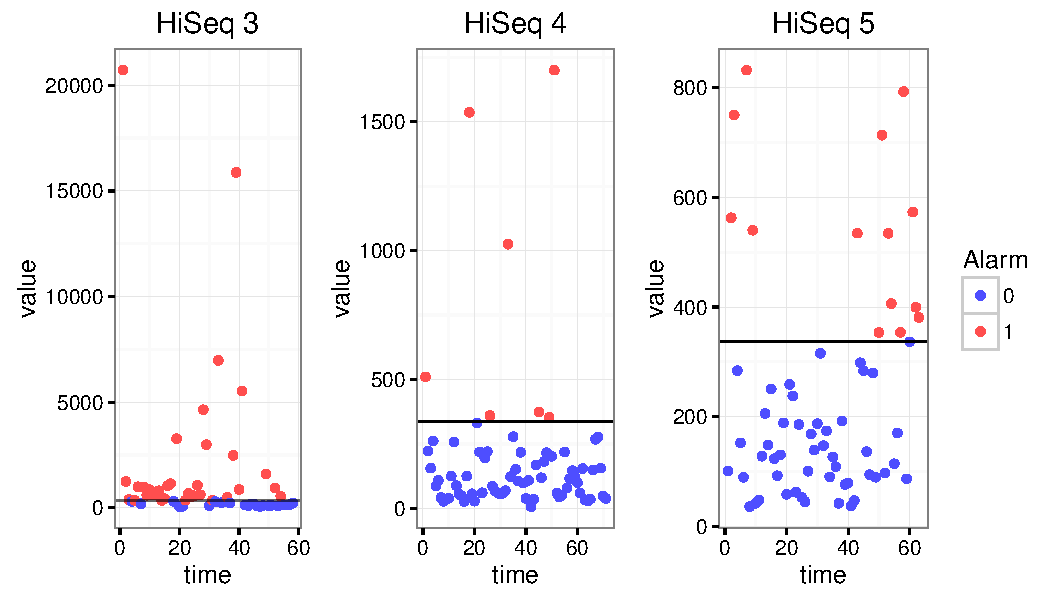
\includegraphics[width=\maxwidth]{figure/HiSeqPhase2Hotelling-1} \caption[Hotellings T-square statistic for the HiSeq 3 (left), HiSeq 4 (middle) and HiSeq 5 machines with in control parameters based on HiSeq 6 data]{Hotellings T-square statistic for the HiSeq 3 (left), HiSeq 4 (middle) and HiSeq 5 machines with in control parameters based on HiSeq 6 data. The straight horizontal line represents the control limit.}\label{fig:HiSeqPhase2Hotelling}
\end{figure}

\begin{kframe}\begin{alltt}
\hlkwd{rm}\hlstd{(p1,p2,p3)}

\hlstd{lambda4} \hlkwb{<-} \hlkwd{t}\hlstd{(mu0}\hlopt{-}\hlkwd{colMeans}\hlstd{(Hiseq4.Trans))}\hlopt\hlstd{Sigma0}\hlopt\hlstd{(mu0}\hlopt{-}\hlkwd{colMeans}\hlstd{(Hiseq4.Trans))}
\hlstd{lambda5} \hlkwb{<-} \hlkwd{t}\hlstd{(mu0}\hlopt{-}\hlkwd{colMeans}\hlstd{(Hiseq5.Trans))}\hlopt\hlstd{Sigma0}\hlopt\hlstd{(mu0}\hlopt{-}\hlkwd{colMeans}\hlstd{(Hiseq5.Trans))}

\hlstd{M1} \hlkwb{<-} \hlkwd{nrow}\hlstd{(Hiseq4.Trans)}
\hlstd{M2} \hlkwb{<-} \hlkwd{nrow}\hlstd{(Hiseq5.Trans)}
\hlstd{detHiseq4}\hlkwb{<-} \hlkwd{det}\hlstd{(}\hlkwd{var}\hlstd{(Hiseq4.Trans)}\hlopt{*}\hlstd{(M1}\hlopt{-}\hlnum{1}\hlstd{)}\hlopt{/}\hlstd{M1)}
\hlstd{detHiseq5}\hlkwb{<-} \hlkwd{det}\hlstd{(}\hlkwd{var}\hlstd{(Hiseq5.Trans)}\hlopt{*}\hlstd{(M2}\hlopt{-}\hlnum{1}\hlstd{)}\hlopt{/}\hlstd{M2)}
\hlstd{detHiseq6}\hlkwb{<-} \hlkwd{det}\hlstd{(Sigma0)}

\hlstd{tmp} \hlkwb{<-} \hlkwd{data.frame}\hlstd{(}\hlstr{"HiSeq 4"} \hlstd{= detHiseq6}\hlopt{/}\hlstd{detHiseq4,} \hlstr{"HiSeq 5"} \hlstd{= detHiseq6}\hlopt{/}\hlstd{detHiseq5)}
\hlcom{#xtable(tmp, label="tab:DetTable", caption="Table containing the Determinant of each estimated covaraince matrix")}
\end{alltt}
\end{kframe}
\end{knitrout}
The MCUSUM charts for the mean vector and covariance matrix are shown in Figure \ref{fig:HiSeq45MCUSUMfig} for the HiSeq 4 and 5 machines. We can see that the charts give a strong indication that the estimated in control mean vector and covariance matrix do not fit the transformed quality data of HiSeq 4 and 5. If we assume that the transformed quality control data for HiSeq 4 and 5 can represent a IC sample from their respective processes, we can calculate the non-centrality parameter, described in section \ref{croiserCUSUM}. Note that we are not removing any observations from the HiSeq 4 and 5 quality control data and that we are using the transformation parameter estimated from HiSeq 6 quality control data. Let $\hat{\boldsymbol{\mu}}_{i}$ be the maximum likelihood estimator of the mean vector based on the $i$'th HiSeq (transformed) quality control data. The non-centrality parameter for HiSeq 4 can be calculated to 
$$
(\hat{\boldsymbol{\mu}}_{0}-\hat{\boldsymbol{\mu}}_{4})\widehat{\Sigma}_0(\hat{\boldsymbol{\mu}}_{0}-\hat{\boldsymbol{\mu}}_{4})'=0.205.
$$
The non-centrality parameter based on HiSeq 5 is calculated to $4.9264789$. The covariance matrices can be compared using the determinant of the covariance matrices. It represents the squared volume of the parallelotope in $\mathcal{R}^p$ where the eigenvectors are the principal edges (cf. \citet[page 385]{MultStatAnalysis}). The ratio of the determinants serve as a measure of how the squared volume of the parallelotope relates to eachother. Let $\widehat{\Sigma}_i$ be the maximum likelihood estimator based on transformed quality control data from the $i$th HiSeq machine. Let
$$
R_{i} = \frac{|\widehat{\Sigma}_0|}{|\widehat{\Sigma}_i|}
$$
be the ratio between the in control covariance matrix and the estimated covariance matrix based on the $i$'th HiSeq transformed quality control data. The ratio $R_{i}$ for HiSeq 4 transformed quality control data is equal to $R_{4}=\ensuremath{3.0064497\times 10^{12}}$ and for HiSeq 5 we have $R_{5}=\ensuremath{5.5434293\times 10^{8}}$. In the transformed space, these covariance matrices are not equal in terms of their parallelotope volume. Note that this only gives a illustration to whether or not their volume is equal. It does not take the inherent structure of the covariance matrix into account. Also, as described in section \ref{Wishartderiv}, any control chart constructed from the transformed quantities would be sensitive to shifts in the mean. The very large values of the charting statistics, seen in the right column of Figure \ref{fig:HiSeq45MCUSUMfig} could be a result of differences in the covariance matrix \textit{and} the mean vector. Since the charts gave a indication of a change in this manner, the change-point detection model will not be used in this setting.
\begin{knitrout}
\definecolor{shadecolor}{rgb}{0.969, 0.969, 0.969}\color{fgcolor}\begin{kframe}
\begin{alltt}
\hlcom{### MCUSUM}
\hlstd{k} \hlkwb{<-} \hlnum{0.3}
\hlstd{covH} \hlkwb{<-} \hlstd{H_ListSigma[[}\hlnum{1}\hlstd{]]}\hlopt{$}\hlstd{Intervals} \hlopt
  \hlkwd{na.omit}\hlstd{()} \hlopt
  \hlkwd{tail}\hlstd{(}\hlnum{1}\hlstd{)} \hlopt
  \hlkwd{mean}\hlstd{()}

\hlstd{meanH} \hlkwb{<-} \hlstd{H_Listmean[[}\hlnum{1}\hlstd{]]}\hlopt{$}\hlstd{Intervals} \hlopt
  \hlkwd{na.omit}\hlstd{()} \hlopt
  \hlkwd{tail}\hlstd{(}\hlnum{1}\hlstd{)} \hlopt
  \hlkwd{mean}\hlstd{()}
\hlstd{ConstructMeanChartingStatistic} \hlkwb{<-} \hlkwa{function}\hlstd{(}\hlkwc{data}\hlstd{) \{}
  \hlcom{# function calculating the charting statistic of the MCUSUM mean}
  \hlstd{ret} \hlkwb{<-} \hlkwd{c}\hlstd{()}
  \hlstd{Sold} \hlkwb{<-} \hlkwd{rep}\hlstd{(}\hlnum{0}\hlstd{,} \hlkwd{ncol}\hlstd{(Sigma0))}


  \hlkwa{for}\hlstd{(i} \hlkwa{in} \hlnum{1}\hlopt{:}\hlkwd{nrow}\hlstd{(data))\{}
    \hlstd{tmp} \hlkwb{<-} \hlkwd{MCUSUM}\hlstd{(}\hlkwc{Snew}\hlstd{=}\hlkwd{unlist}\hlstd{(data[i,]),}\hlkwc{Sold} \hlstd{= Sold,} \hlkwc{mu0}\hlstd{=mu0,} \hlkwc{Sigma0} \hlstd{= Sigma0,} \hlkwc{k}\hlstd{=k)}

    \hlstd{Sold} \hlkwb{<-} \hlstd{tmp}\hlopt{$}\hlstd{Snew}
    \hlstd{Cstat} \hlkwb{<-} \hlstd{tmp}\hlopt{$}\hlstd{Cstatistic}
    \hlstd{ret} \hlkwb{<-} \hlkwd{c}\hlstd{(ret,Cstat)}
  \hlstd{\}}
  \hlkwd{return}\hlstd{(ret)}
\hlstd{\}}
\hlcom{### Wishart transformation}
\hlstd{ConstructWishartChartingStatistic}\hlkwb{<-} \hlkwa{function}\hlstd{(}\hlkwc{data}\hlstd{) \{}
  \hlcom{# Function which construct the charting statistic for the Wishart distribution.}

  \hlcom{# Args: }
  \hlcom{# data: (data.frame) data.frame on the same format as the initial data which was used to estimate mu0 and sigma0.}
  \hlstd{ret} \hlkwb{<-} \hlkwd{c}\hlstd{()}
  \hlstd{Sold} \hlkwb{<-} \hlkwd{rep}\hlstd{(}\hlnum{0}\hlstd{,} \hlkwd{ncol}\hlstd{(Sigma0)}\hlopt{-}\hlnum{1}\hlstd{)}

  \hlkwa{for} \hlstd{(j} \hlkwa{in} \hlnum{1}\hlopt{:}\hlkwd{nrow}\hlstd{(data))\{}
    \hlstd{tmp} \hlkwb{<-} \hlkwd{lapply}\hlstd{(}\hlnum{1}\hlopt{:}\hlkwd{ncol}\hlstd{(data),}\hlkwa{function}\hlstd{(}\hlkwc{x}\hlstd{)} \hlkwd{TransformObsWishart}\hlstd{(}\hlkwc{observation}\hlstd{=}\hlkwd{unlist}\hlstd{(data[j,]),}\hlkwc{i}\hlstd{=x,}\hlkwc{mu0}\hlstd{=mu0,}\hlkwc{sigma0} \hlstd{= Sigma0))}
    \hlstd{WhichMaxStatistic} \hlkwb{<-} \hlkwd{lapply}\hlstd{(tmp,} \hlkwa{function}\hlstd{(}\hlkwc{x}\hlstd{)} \hlkwd{MCUSUM}\hlstd{(}\hlkwc{Snew}\hlstd{=x,}\hlkwc{Sold}\hlstd{=Sold,}\hlkwc{mu0}\hlstd{=}\hlkwd{rep}\hlstd{(}\hlnum{0}\hlstd{,}\hlkwd{ncol}\hlstd{(Sigma0)}\hlopt{-}\hlnum{1}\hlstd{),}\hlkwc{Sigma0} \hlstd{=} \hlkwd{diag}\hlstd{(}\hlkwd{ncol}\hlstd{(Sigma0)}\hlopt{-}\hlnum{1}\hlstd{),} \hlkwc{k}\hlstd{=k)}\hlopt{$}\hlstd{Cstatistic)} \hlopt
      \hlkwd{unlist}\hlstd{()} \hlopt
      \hlkwd{which.max}\hlstd{()}

    \hlstd{tmp} \hlkwb{<-} \hlkwd{MCUSUM}\hlstd{(}\hlkwc{Snew}\hlstd{=tmp[[WhichMaxStatistic]],}\hlkwc{Sold}\hlstd{=Sold ,}\hlkwc{mu0}\hlstd{=}\hlkwd{rep}\hlstd{(}\hlnum{0}\hlstd{,}\hlkwd{ncol}\hlstd{(Sigma0)}\hlopt{-}\hlnum{1}\hlstd{),} \hlkwc{Sigma0} \hlstd{=} \hlkwd{diag}\hlstd{(}\hlkwd{ncol}\hlstd{(Sigma0)}\hlopt{-}\hlnum{1}\hlstd{),} \hlkwc{k}\hlstd{=k)}
    \hlstd{Sold} \hlkwb{<-} \hlstd{tmp}\hlopt{$}\hlstd{Snew}

    \hlstd{Hstatistic} \hlkwb{<-} \hlstd{tmp}\hlopt{$}\hlstd{Cstatistic}
    \hlstd{ret} \hlkwb{<-} \hlkwd{c}\hlstd{(ret,Hstatistic)}
  \hlstd{\}}
  \hlkwd{return}\hlstd{(ret)}
\hlstd{\}}

\hlcom{#### MCUSUM mean}
\hlstd{Mean_HiSeq4} \hlkwb{<-}  \hlkwd{data.frame}\hlstd{(}\hlstr{"HiSeq4"}\hlstd{=}\hlkwd{ConstructMeanChartingStatistic}\hlstd{(Hiseq4.Trans),}
                           \hlstr{"x"}\hlstd{=}\hlnum{1}\hlopt{:}\hlkwd{nrow}\hlstd{(Hiseq4.Trans),}
                           \hlstr{"Alarm"}\hlstd{=}\hlkwd{as.factor}\hlstd{(}\hlkwd{ifelse}\hlstd{(}\hlkwd{ConstructMeanChartingStatistic}\hlstd{(Hiseq4.Trans)}\hlopt{>}\hlstd{meanH,}\hlnum{1}\hlstd{,}\hlnum{0}\hlstd{)))}

\hlstd{Mean_HiSeq5} \hlkwb{<-}  \hlkwd{data.frame}\hlstd{(}\hlstr{"HiSeq5"}\hlstd{=}\hlkwd{ConstructMeanChartingStatistic}\hlstd{(Hiseq5.Trans),}
                           \hlstr{"x"}\hlstd{=}\hlnum{1}\hlopt{:}\hlkwd{nrow}\hlstd{(Hiseq5.Trans),}
                           \hlstr{"Alarm"}\hlstd{=}\hlkwd{as.factor}\hlstd{(}\hlkwd{ifelse}\hlstd{(}\hlkwd{ConstructMeanChartingStatistic}\hlstd{(Hiseq5.Trans)}\hlopt{>}\hlstd{meanH,}\hlnum{1}\hlstd{,}\hlnum{0}\hlstd{)))}
\hlcom{#### MCUSUM Wishart.}
\hlstd{Wishart_Hiseq4} \hlkwb{<-} \hlkwd{data.frame}\hlstd{(}\hlstr{"HiSeq4"}\hlstd{=}\hlkwd{ConstructWishartChartingStatistic}\hlstd{(Hiseq4.Trans),}
                             \hlstr{"x"}\hlstd{=}\hlnum{1}\hlopt{:}\hlkwd{nrow}\hlstd{(Hiseq4.Trans),}
                             \hlstr{"Alarm"}\hlstd{=}\hlkwd{as.factor}\hlstd{(}\hlkwd{ifelse}\hlstd{(}\hlkwd{ConstructWishartChartingStatistic}\hlstd{(Hiseq4.Trans)}\hlopt{>}\hlstd{covH,}\hlnum{1}\hlstd{,}\hlnum{0}\hlstd{)))}
\hlstd{Wishart_Hiseq5} \hlkwb{<-} \hlkwd{data.frame}\hlstd{(}\hlstr{"HiSeq5"}\hlstd{=}\hlkwd{ConstructWishartChartingStatistic}\hlstd{(Hiseq5.Trans),}
                             \hlstr{"x"}\hlstd{=}\hlnum{1}\hlopt{:}\hlkwd{nrow}\hlstd{(Hiseq5.Trans),}
                             \hlstr{"Alarm"}\hlstd{=}\hlkwd{as.factor}\hlstd{(}\hlkwd{ifelse}\hlstd{(}\hlkwd{ConstructWishartChartingStatistic}\hlstd{(Hiseq5.Trans)}\hlopt{>}\hlstd{covH,}\hlnum{1}\hlstd{,}\hlnum{0}\hlstd{)))}
\end{alltt}
\end{kframe}
\end{knitrout}

\begin{knitrout}
\definecolor{shadecolor}{rgb}{0.969, 0.969, 0.969}\color{fgcolor}\begin{kframe}
\begin{alltt}
\hlstd{p1} \hlkwb{<-} \hlkwd{ggplot}\hlstd{(Mean_HiSeq4)} \hlopt{+}
  \hlkwd{geom_point}\hlstd{(}\hlkwd{aes}\hlstd{(}\hlkwc{x}\hlstd{=x,}\hlkwc{y}\hlstd{=HiSeq4,} \hlkwc{color}\hlstd{=Alarm))} \hlopt{+}
  \hlkwd{geom_hline}\hlstd{(}\hlkwc{yintercept}\hlstd{=meanH)} \hlopt{+}
  \hlkwd{ylab}\hlstd{(}\hlstr{"value"}\hlstd{)} \hlopt{+}
  \hlkwd{xlab}\hlstd{(}\hlstr{"time"}\hlstd{)} \hlopt{+}
  \hlkwd{theme_bw}\hlstd{()} \hlopt{+}
  \hlkwd{scale_color_manual}\hlstd{(}\hlstr{" "}\hlstd{,} \hlkwc{values} \hlstd{=} \hlkwd{c}\hlstd{(}\hlstr{"#4e4eff"}\hlstd{,}\hlstr{"#ff4e4e"}\hlstd{),} \hlkwc{breaks}\hlstd{=}\hlkwd{c}\hlstd{(}\hlstr{"Alarm"}\hlstd{,}\hlstr{"No Alarm"}\hlstd{))} \hlopt{+}
  \hlkwd{ggtitle}\hlstd{(}\hlstr{"HiSeq 4 - Mean"}\hlstd{)}

\hlstd{p11} \hlkwb{<-} \hlkwd{ggplot}\hlstd{(Mean_HiSeq5)} \hlopt{+}
  \hlkwd{geom_point}\hlstd{(}\hlkwd{aes}\hlstd{(}\hlkwc{x}\hlstd{=x,}\hlkwc{y}\hlstd{=HiSeq5,} \hlkwc{color}\hlstd{=Alarm))} \hlopt{+}
  \hlkwd{geom_hline}\hlstd{(}\hlkwc{yintercept}\hlstd{=meanH)} \hlopt{+}
  \hlkwd{ylab}\hlstd{(}\hlstr{"value"}\hlstd{)} \hlopt{+}
  \hlkwd{xlab}\hlstd{(}\hlstr{"time"}\hlstd{)} \hlopt{+}
  \hlkwd{theme_bw}\hlstd{()} \hlopt{+}
  \hlkwd{scale_color_manual}\hlstd{(}\hlstr{" "}\hlstd{,} \hlkwc{values} \hlstd{=} \hlkwd{c}\hlstd{(}\hlstr{"#4e4eff"}\hlstd{,}\hlstr{"#ff4e4e"}\hlstd{),} \hlkwc{breaks}\hlstd{=}\hlkwd{c}\hlstd{(}\hlstr{"Alarm"}\hlstd{,}\hlstr{"No Alarm"}\hlstd{))} \hlopt{+}
  \hlkwd{ggtitle}\hlstd{(}\hlstr{"HiSeq 5 - Mean"}\hlstd{)}

\hlstd{p2} \hlkwb{<-} \hlkwd{ggplot}\hlstd{(Wishart_Hiseq4)} \hlopt{+}
  \hlkwd{geom_point}\hlstd{(}\hlkwd{aes}\hlstd{(}\hlkwc{x}\hlstd{=x,}\hlkwc{y}\hlstd{=HiSeq4,} \hlkwc{color}\hlstd{=Alarm))} \hlopt{+}
  \hlkwd{geom_hline}\hlstd{(}\hlkwc{yintercept}\hlstd{=covH)} \hlopt{+}
  \hlkwd{ylab}\hlstd{(}\hlstr{"value"}\hlstd{)} \hlopt{+}
  \hlkwd{xlab}\hlstd{(}\hlstr{"time"}\hlstd{)} \hlopt{+}
  \hlkwd{theme_bw}\hlstd{()} \hlopt{+}
  \hlkwd{scale_color_manual}\hlstd{(}\hlstr{""}\hlstd{,} \hlkwc{values} \hlstd{=} \hlkwd{c}\hlstd{(}\hlstr{"#ff4e4e"}\hlstd{),} \hlkwc{breaks}\hlstd{=}\hlkwd{c}\hlstd{(}\hlstr{"Alarm"}\hlstd{))} \hlopt{+}
  \hlkwd{ggtitle}\hlstd{(}\hlstr{"HiSeq 4 - Covariance"}\hlstd{)}

\hlstd{p22} \hlkwb{<-} \hlkwd{ggplot}\hlstd{(Wishart_Hiseq5)} \hlopt{+}
  \hlkwd{geom_point}\hlstd{(}\hlkwd{aes}\hlstd{(}\hlkwc{x}\hlstd{=x,}\hlkwc{y}\hlstd{=HiSeq5,} \hlkwc{color}\hlstd{=Alarm))} \hlopt{+}
  \hlkwd{geom_hline}\hlstd{(}\hlkwc{yintercept}\hlstd{=covH)} \hlopt{+}
  \hlkwd{ylab}\hlstd{(}\hlstr{"value"}\hlstd{)} \hlopt{+}
  \hlkwd{xlab}\hlstd{(}\hlstr{"time"}\hlstd{)} \hlopt{+}
  \hlkwd{theme_bw}\hlstd{()} \hlopt{+}
  \hlkwd{scale_color_manual}\hlstd{(}\hlstr{""}\hlstd{,} \hlkwc{values} \hlstd{=} \hlkwd{c}\hlstd{(}\hlstr{"#ff4e4e"}\hlstd{),} \hlkwc{breaks}\hlstd{=}\hlkwd{c}\hlstd{(}\hlstr{"Alarm"}\hlstd{))} \hlopt{+}
  \hlkwd{ggtitle}\hlstd{(}\hlstr{"HiSeq 5 - Covariance"}\hlstd{)}

\hlkwd{grid.arrange}\hlstd{(p1,p2, p11,p22,} \hlkwc{ncol}\hlstd{=}\hlnum{2}\hlstd{)}
\end{alltt}
\end{kframe}\begin{figure}
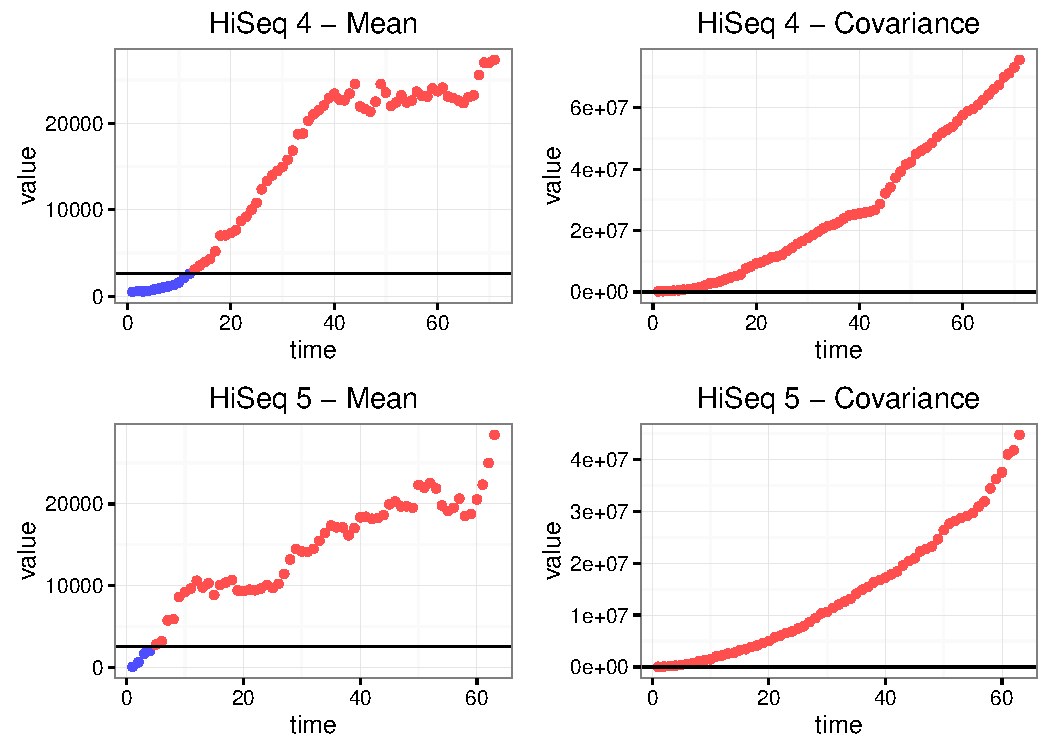
\includegraphics[width=\maxwidth]{figure/HiSeq45MCUSUMfig-1} \caption[MCUSUM control charts monitoring the mean vector and covariance matrix]{MCUSUM control charts monitoring the mean vector and covariance matrix. The in control parameters is based on transformed data from the HiSeq 6 machine. The horizontal line is the control limit calculated with k=0.3.}\label{fig:HiSeq45MCUSUMfig}
\end{figure}


\end{knitrout}

\bibliography{REFERENCES.bib}
\end{document}
